\chapter{Aim}
\label{chap:aim}
ASD is a disorder that has been increased in the population in the last years. The main reason for that  is that methods for discover ASD has been improved and knowledge about the disorder has expand and child care personnel has been educate to look for symptoms in early stage of the child's development. %(https://www.fhi.no/fp/barn-og-unge/utviklingsforstyrrelser/autisme---faktaark/)
Various research is done to highlight methods (reference) discovering ASD and to emphasize ASD therapy possibilities. Nowadays,  standard evaluation tests like M-ABC2, MOT4-5, BOT2 are used by psychologist in order to determine ASD disorder of a child.
(http://entwicklungsdiagnostik.de/m-abc-2.html)
These tests evaluate  the ability of motor-coordination of children, divided in different age groups, in a  in form of hand dexterity, balance and ball skills.
Furthermore, research showed that children with ASD have disruption of normal movement pattern which also is indication of motor coordination deficit.(reference).

According to (reference), test methods that could determine ASD are expensive, time consuming and demand a laboratory environment. 

The idea of this project is to determine whether Leap motion and hand gesture software could be used as a supplementary evaluation and screening tool for ASD in health and education sector. The benefits of using Leap Motion are many, as for instance the portability and low acquisition cost. The evaluation can happen anywhere , even in an environment where kids feel comfortable and  familiar. (Laboratories are artificial environment which other impact can be controlled but on the other side can make children uncomfortable. Children feel more secure in an known environment. (find REFERENCE)
The Leap motion sensor could than not only be use as a screening method but also as a therapy tool for fine motor exercises.


Leap Motion is a sensor for gesture control. It is used to control software with hand and finger gesture. Nowadays, evaluation exercises  are more or less analogical, (interview) as descripted in “Entwicklingsdiagnostik.de”. (http://entwicklungsdiagnostik.de/m-abc-2.html) A more up to date evaluation teknik would be digital. Since Leap motion can screen fine motoric movements, it would be a suitable evaluation tool that is enjoyable, accessible and economical.


The research of this master thesis will focus on performance measurement of eye-hand coordination (EHC) on young children(define young?) and investigate in what degree Leap Motion sensor and free-hand gesture based games (or/and gesture controlled tools such as Arduino smartcar ) are a convenient measurement tool in order to determine ASD in a early stage. In addition, the research will explore if those tools are appropriate for ergo- and physiotherapeutic use for young children with fine-motoric problems.

In order to fulfill the requirement of  LP sensor and gesture software game as an ASD evaluation tool, these technology must address several parameters. As mentioned the chapter (ASD) the disorder is marked by several deficits such as motor-coordination deficit, sensorimotor deficit, motor timing disruption, psychomotor deficit that are essential when using LP as a evaluation tool. 

The hand-free gesture evaluation tool is a software that uses Leap Motion sensor which functions as a supplementary evaluation tool. The software has 5 modules  and each one checks the capacity of motor coordination and hand dexterity of children.
\vspace{5mm} %5mm vertical space
\hfill \break
Module 1 - Ladybug\newline
Task description: The goal of this task is to put as many ladybugs on a three a possible in a certain time frame. The child has to move a ladybug from the ground up to the tree by only his/her index finger.
Evaluation parameters: count the amount of bug are move in a given time period
Based on: M-ABC2 ( insert coins task)
\vspace{5mm} %5mm vertical space
\hfill \break
Module 2 - Flying balloon\newline
Task description: Flying balloon is a pointing game where the participant must hit the balloons in order to burst them. The balloons are moving over the screen entirely arbitrary. The goal is to burst as many balloon as possible in a certain time period.
Evaluation parameters: Hand eye coordination, accuracy and timing
Based on: M-ABC2 
\vspace{5mm} %5mm vertical space
\hfill \break
Module 3 - Mole in the hole\newline
Task description: The goal of this game is to guide the mole out of his hole. This is a precision game which demands concentration and patience 
Evaluation parameters:  precision, concentration, patience 
Based on: M-ABC2 for hand dexterity test - trace a track
\vspace{5mm} %5mm vertical space
\hfill \break
Module 4 - MEMO \newline
Task description: The game builds on the participants memory ability.  The participant will see a row of objects and the corresponding gestures for a certain amount of time. The participant has to memorize the gesture belonging to the object. Than the object appears on the screen and the participant has to remember the appropriate gesture. 
Evaluation parameters: remember and recall. This is a cognitive task for testing of psychomotor deficit.
Based on:
\vspace{5mm} %5mm vertical space
\hfill \break
Module 5 - Freehand drawing\newline
Task description: In this game the participant is asked to draw a shape with a the pointing finger.  The participant will see a shape on the screen and needs to repeat the drawing. The participant could also be ask to make an existing shape smaller or bigger by pinch movements.
Evaluation parameters: fine motor coordination
Based on standard tool: DMB ( trace geometrical forms) and LOS ( paint circles in the air)

\vspace{5mm} %5mm vertical space
\hfill \break
To sum up autism is defined by:
\begin{itemize}
    \item Motor-coordination deficit
    \item Sensory deficit
    \item Motor-timing disruption
    \item Psycho-motor deficit
    \item Disruption of normal movement pattern
\end{itemize}


%\begin{center}
%\begin{tabular}{|c|c|c|c|c| }%| m{1cm}| m{1cm} |  m{1cm} | %m{1cm} | m{1cm}|} 
% \hline
% Parameters - identify ASD & Task description & Deficit/
%Disruption & LM parameters &  Game/task \\ 
% \hline
% \hline
% cell7 & cell8 & cell9 & cell8 & cell9 \\ 
% \hline
%\end{tabular}
%\end{center}

\begin{figure}[h]  %t top, b bottom, p page | you can also use h to try to get the figure to appear at the current location
  
  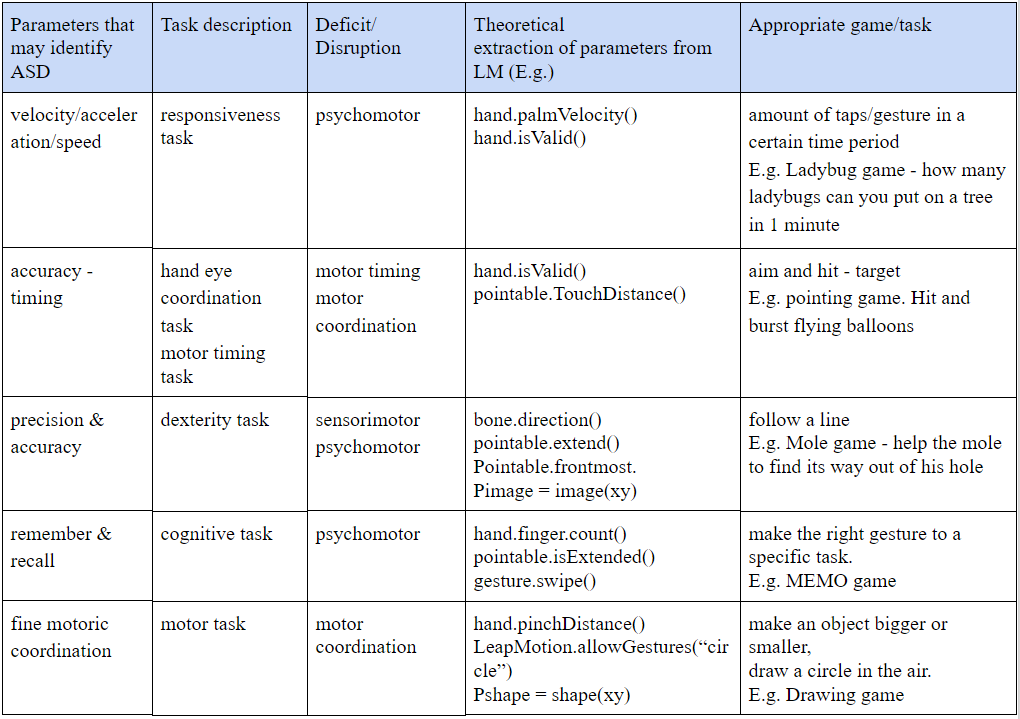
\includegraphics[width=1\textwidth]{figures/tableOfModules.png}
  \caption[Parameters and Modules.]{Parameters and Modules.}
  \label{fig:setup}
\end{figure}


\section{Research Question}
\label{sec:researchquestion}


\section{Hypothesis}
\label{sec:hypothesis}


